\Main
\hspace{0pt}
\vfill
\begin{center}
ОСНОВНАЯ ЧАСТЬ
\end{center}
\vfill
\hspace{0pt}
\pagebreak

\chapter{Теоретическая часть}
\label{cha:ch_1}

\section{Постановка задачи}
В рамках данной выпускной квалификационной работы предполагается выбрать
компоненты для реализации и разработать инфраструктуру по поиску алгоритмов.

Инфраструктуру в целом требуется разработать в соответствии концепции
микросервисной архитектуры. Плюсом такой реализации является легкая заменяемость
модулей. Также необходимо средство контейнеризации и оркестрации контейнеров.
Необходимо для более легкого развертывания приложений на облачных структурах
(вычислительных серверах).

Логика инфраструктуры будет заключаться в следующем:
\begin{enumerate}[label=\arabic*.]
    \item Считать запрос пользователя. Т.е. предложить ему выбор вписать желаемое самому или выбрать из списка доступных опций;
    \item Произвести поиск по ключевым словам на необходимых интернет ресурсах;
    \item Выделить из возвращенных html страниц необходимые данные (произвести уточняющие запросы, либо запросы перехода на следующую страницу пагинации, если требуется);
    \item Полученные данные положить в базу данных;
    \item Пользователь теперь имеет возможность посмотреть, что нашлось.
\end{enumerate}

\section{Микросервисная архитектура}
Для разработки приложения для данной выпускной квалификационной работы была выбрана микросервисная архитектура.
% https://ru.wikipedia.org/wiki/%D0%9C%D0%B8%D0%BA%D1%80%D0%BE%D1%81%D0%B5%D1%80%D0%B2%D0%B8%D1%81%D0%BD%D0%B0%D1%8F_%D0%B0%D1%80%D1%85%D0%B8%D1%82%D0%B5%D0%BA%D1%82%D1%83%D1%80%D0%B0
Микросервисная архитектура - такой вариант сервис-ориентированной архитектуры
программного обеспечения, который направлен на взаимодействие наиболее
раздробленных, небольших, слабосвязанных и легко модифицируемых модулей, которые
называются микросервисами.

У данной архитектуры есть ряд преимуществ и недостатков. Начнем с преимуществ:
\begin{itemize}
    \item модули (из которых состоит инфраструктура) легко заменяемые (не нужно
        полностью пересобирать и развертывать всю инфраструктуру, при внесении
        небольших изменений);
    \item сервисы могут быть реализованны с помощью разных средств, где
        последние выбираются в пользу высокой эффективности;
    \item архитектура получается симметричная, а не иерархическая.
\end{itemize}

Нельзя обойтись и без недостатков:
\begin{itemize}
    \item Сложность начальной разработки;
    \item Могут возникать сетевые издержки;
    \item Формат сообщений между сервисами должен быть стандартизован, что
        приводит к дополнительным издержкам на поддержание инфраструктуры.
\end{itemize}

% «Создание микросервисов», Сэм Ньюмен, стр 23
Микросервисная архитектура также хорошо отвечает принципу единственной
обязанности -- Single Rsponsibility Principle, которое гласит: «Собирайте вместе
все, что изменяется по одной и той же причине и разделяйте все, что изменяется
по разным причинам».

% https://mcs.mail.ru/blog/prostym-jazykom-o-mikroservisnoj-arhitekture
Для сравнения, в монолитной архитектуре все компоненты соеденены в единое целое.
Вся логика по обработке запросов помещается внутрь одного процесса. Разумеется,
монолиты могут иметь модульную стркутуру -- содержать отдельные классы, функции.
Но связи между этими модулями настолько сильны, что изменение каждого из них
неизбежно отражается на работе приложения в целом.
\begin{figure}[H]
    \centering
    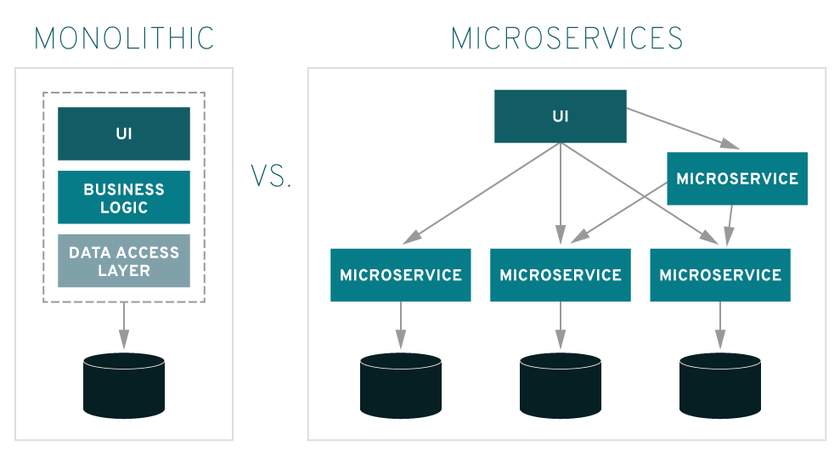
\includegraphics[scale=0.6]{inc/img/Monolithic-vs-microservices.png}
    \caption{Сравнение микросервисной и монолитной архитектуры}
\end{figure}

\section{Технология контейнеризации}
% https://ru.wikipedia.org/wiki/%D0%92%D0%B8%D1%80%D1%82%D1%83%D0%B0%D0%BB%D0%B8%D0%B7%D0%B0%D1%86%D0%B8%D1%8F
По определению виртуализация -- это предоставление набора вычислительных
ресурсов или их логического объединения, абстрагированное от аппаратной
реализации, и обеспечивающее при этом логическую изоляцию друг от друга
вычислительных процессов, выполняемых на одном физическом ресурсе.

% https://habr.com/ru/company/southbridge/blog/530226/
% https://eternalhost.net/blog/razrabotka/docker-kubernetes
Одной из отличительных черт контейнеров от виртуальных машин -- то, что первые
используют возможность не железа, а операционной системы, так называемое
пространство имен. Можно произвести грубое сравнение виртуальных машин и
контейнеров:
% learning docker
\begin{table}[H]
    \centering
    \begin{tabular}{|l|l|}
        \hline
        {\bf Виртуальные машины}                   & {\bf Контейнеры} \\\hline
        Аппаратная виртуализация                   & Виртуализация на уровне ОС \\\hline
        Тяжеловесные                               & Легковесные \\\hline
        Полностью изолированные (более безопасные) & Изолирование на уровне процессов \\\hline
    \end{tabular}
    \caption{Сравнение виртуальных машин и контейнеров}
\end{table}
\begin{figure}[H]
    \centering
    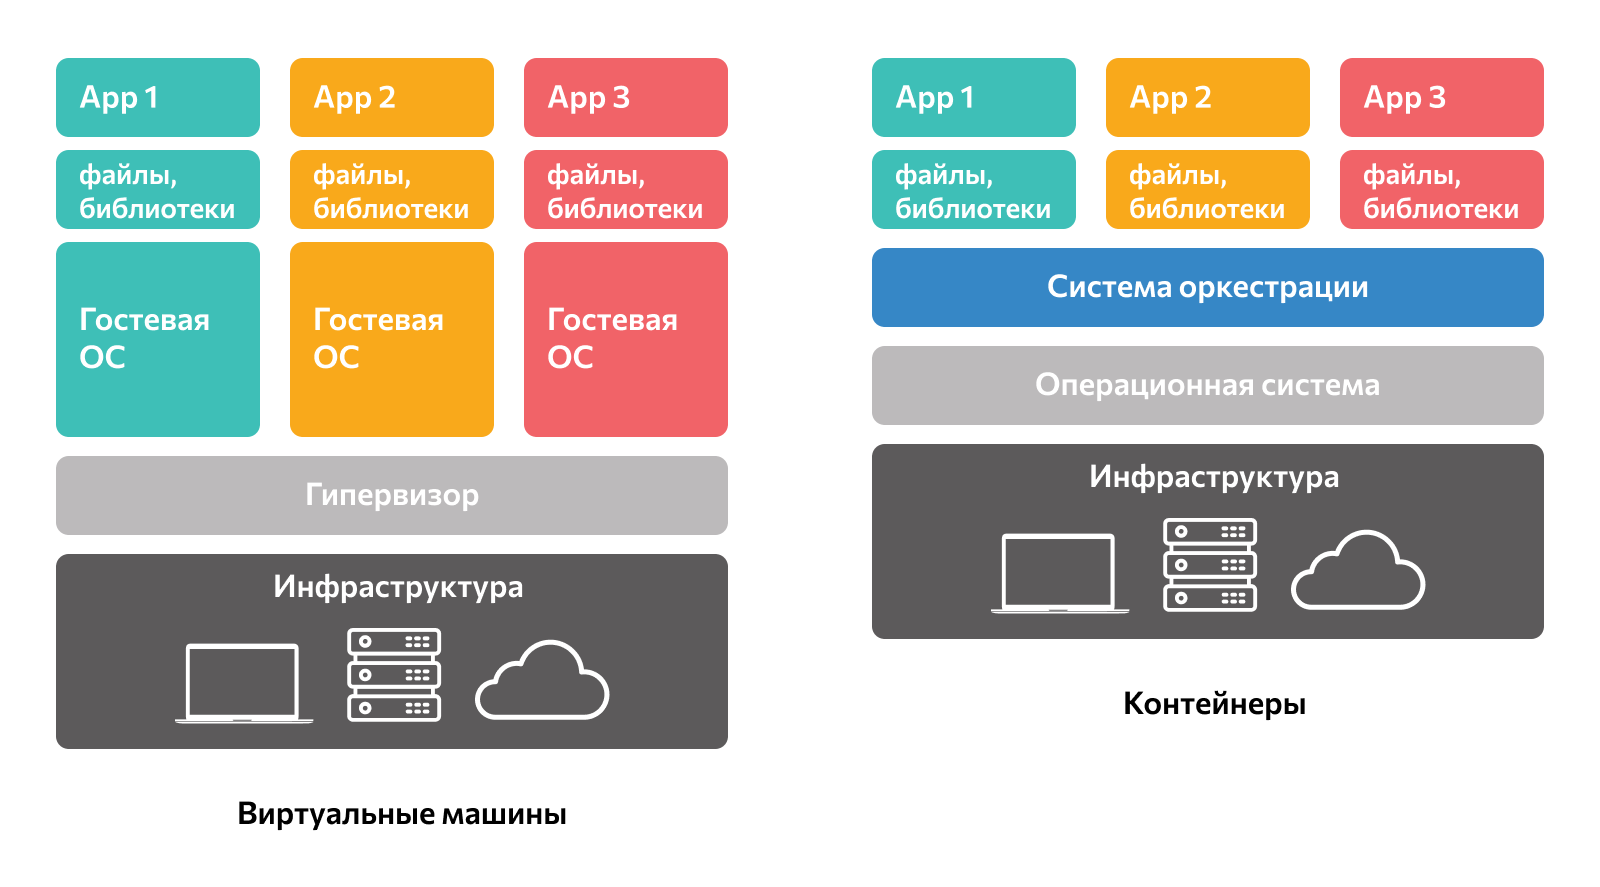
\includegraphics[scale=0.25]{inc/img/cont-vs-virt.png}
    \caption{Сравнение виртуальных машин и контейнеров}
\end{figure}

% https://blog.skillfactory.ru/glossary/kontejnerizacziya/
Технологии контейнеризации решают проблему изолированного запуска приложений и
рабочих сред вне зависимости от системы (должно быть то же ядро) и ПО,
установленных на конкретной машине. Также данная технология позволяет легко
управлять сложными приложениями и средами (упаковывать зависимости, перемещать
решение с системы на систему). 

% TODO: сравнение технологий контейнеризации
\section{Поиск по web-ресурсам}
Для поиска по web-ресурсам безусловно достаточно только возможность совершать
HTTP-запросы (с необходимыми заголовками, сертификатами и т.д.) и читать то, что
сервер возвращает клиенту. Но в целях данной выпускной квалификационной работы
присутствует задача выбрать хорошую архитектуру. Поэтому нужно рассмотреть
фреймворки (или системы), которые позволяют упростить эту самую работу.

% https://pythobyte.com/10-tips-to-avoid-getting-blocked-while-scraping-websites-ncf-bee5b81c/
Также многие сайты стараются скрыть свою информацию от web-ботов. Возможно это
обусловленно тем, что последние злоупотребляют общедоступной информацией либо
вычислительной мощностью, которую сервер выделяет на пользователя. Поэтому, на
таких серверах могут быть настроенны политики запрета доступа к контенту при
слишком частом запросе страницы.

% https://coderlessons.com/tutorials/devops/uchitsia-scrapy/scrapy-kratkoe-rukovodstvo
Свойства которыми должен обладать фреймворк при работе с web-ресурсами:
\begin{itemize}
    \item Быть масштабируемым на большие проекты сканирования;
    \item Асинхронная обработка запросов;
    % TODO: сделать сноску на селекторы
    \item Встроенный механизм работы с селекторами;
    % TODO: сделать сноску на дросселирование
    \item Обладает механизмом автоматического дросселирования;
    \item Генерация результатов в разных структурных текстовых форматах.
\end{itemize}

% сравнение requests, beautiful soup 4, lxml, selenium, scrapy

Фреймворк на python -- scrapy удовлетворяет всем вышеперечисленным свойствам.
Более того для него написанна серверная часть scrapyd, которая позволяет
размещать "пауков" на мощных серверах, с последующим запуском либо по
расписанию, либо по http-запросу.
\begin{figure}[H]
    \centering
    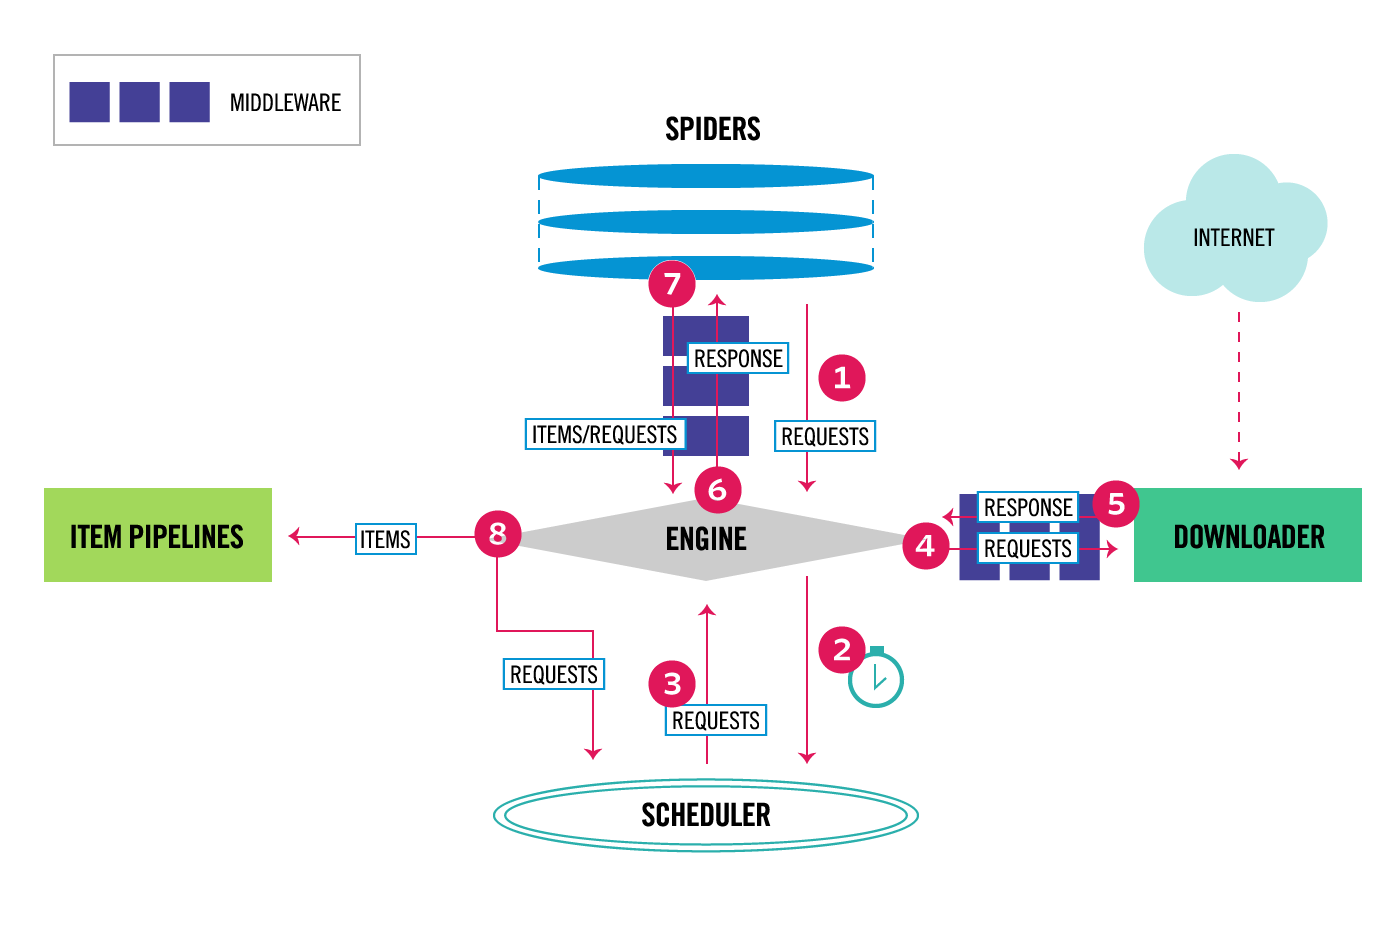
\includegraphics[scale=0.35]{inc/img/scrapy_architecture.png}
    \caption{Архитектура scrapy}
\end{figure}

% TODO: сделать сноску что этот файл обозначает
Также в этом модуле можно настроить много других политик доступа к интернет ресурсам. В такие политики входят:
\begin{itemize}
    \item Чтение файла \verb|robots.txt|;
    \item Лист прокси;
    \item Ротация заголвков и куков.
\end{itemize}

Данная библиотека позволяет полностью посмотреть список настроек, добавить свои,
и написать такую конфигурацию системы, чтобы не добавить свою вычислительную
сеть в черный список целевой структуры.

\section{Серверная часть}
% кто-то читает порт и является в то же время прокси: nginx
% uwsgi: передает сообщения на python
% flask: построен на основе uwsgi для того чтобы просто принимать сообщения, а
% сам является обработчиком

\section{Брокер сообщений}
\section{База данных}

